\chapter{Thiết kế Khả kiểm bằng Phương pháp Quét (Design for Test by Means of Scan)}

(Dịch và biên soạn chi tiết từ: \textbf{7 Design for Test by Means of Scan}, kết hợp bổ sung phân tích chuyên sâu).

\section{Nhập môn và Khái niệm MUX-DFF (Phần Bổ sung của Nhóm)}
\textbf{[Bổ sung kiến thức]} Trước khi đi vào các kỹ thuật phân tích của tài liệu gốc, ta cần hiểu bản chất vật lý của phương pháp Quét (Scan). Trong thiết kế vi mạch truyền thống, việc kiểm thử các mạch tuần tự rất phức tạp do tính chất "nhớ" trạng thái của hàm Flip-Flop. Phương pháp Quét giải quyết vấn đề bằng cách thay thế các D-Flip-Flop (DFF) thông thường thành các Scan Flip-Flop (MUX-DFF). 

\begin{figure}[!ht]
    \centering
    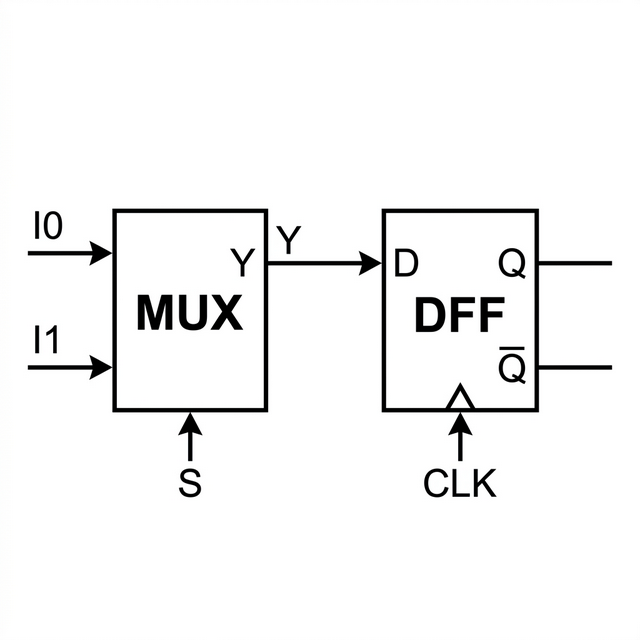
\includegraphics[width=0.6\textwidth]{images/mux_dff.png}
    \caption{Mô hình một Scan Flip-Flop (MUX-DFF) chuẩn được nhóm phân tích}
    \label{fig:mux_dff}
\end{figure}

Như thể hiện ở Hình \ref{fig:mux_dff}, một bộ ghép kênh (MUX) được bổ sung trước ngõ logic D. Nhờ chân điều khiển \texttt{Scan Enable (SE)} hay \texttt{NbarT}, mạch có thể hoán đổi giữa chế độ Normal (mạch hoạt động bình thường cấp dữ liệu logic) và chế độ Shift (kết nối tất cả các Flip-flop thành một thanh ghi dịch dằng dặc). Điều này biến mạch từ "tuần tự" thành "tổ hợp ảo" trong lúc test.

\section{Kiểm thử Quét Toàn cục trên Adding Machine (Full scan Adding Machine)}

Với cơ chế quét (scan) được chèn vào như đã trình bày (ở Hình 7.52 trong tài liệu gốc: \textit{Full scan Adding Machine}), đường dẫn \texttt{data\_bus\_in} trở thành ngõ vào chính (primary input) của mạch, và \texttt{data\_bus\_out} cùng với \texttt{ad\_bus} hợp lại tạo thành cụm ngõ ra chính (primary output). Bản thiết kế mạch khả kiểm này sở hữu 24 ngõ vào giả định (pseudo primary input) và 24 ngõ ra giả định (pseudo primary output), lần lượt tương ứng với các ngõ ra và ngõ vào của thanh ghi hiện hữu.

Để tiến hành kiểm thử mạch này, một mô hình được "trải phẳng" (unfolded model) của toàn mạch đã được tạo ra, hoàn toàn tương tự như cách chúng ta đã làm cho ví dụ Residue-5 ở Mục 7.3. Netlist tổ hợp (combinational netlist) này được sử dụng cho quá trình tự động tổng hợp mẫu thử ATPG bằng công cụ \textbf{HOPE} nhằm nhắm tới 976 điểm lỗi (faults). 

Kết quả là HOPE đã tạo ra 64 vector kiểm thử (\textit{test vectors}) và mang về mức độ bao phủ lỗi (fault coverage) đạt định mức 80.53\%. Mỗi test vector bao gồm 32 bit ở phía ngõ vào và 38 bit ở phía ngõ ra. Từ 32 bit ngõ vào được sinh ra, 8 bit được sử dụng cho \texttt{data\_bus\_in} và 24 bit còn lại được kéo nối thẳng cấp cho đường dẫn quét (scan path). Tương tự ở chiều ngược lại, các số lượng bit ngõ ra lần lượt là 8, 6 và 24 bit tương ứng chỉ định cho \texttt{data\_bus\_out}, \texttt{ad\_bus} và đường scan path thu lượm.

Mô hình khả kiểm hoàn chỉnh của cỗ máy \textit{Adding Machine} thu được bằng cách xâu chuỗi ráo riết tất cả các flip-flop của hệ mạch lại thành một chuỗi (chain) thẳng tắp duy nhất. Hình \ref{lst:753} trình bày bộ kiểm thử ảo (virtual tester) chuyên dùng cho việc kiểm thử full scan trên cấu trúc netlist khả kiểm của mạch này. Đoái hoài ngoại trừ việc thiết bị dưới vòng kiểm thử mạch (circuit under test) mang hình hài khác biệt, và số lượng phép dịch cấp (shifts) trong các scan flip-flop có sự suy xuyển, bộ tester này hoàn toàn không có mảy may phân biệt nào so với bộ tester của mạch Residue-5 được thảo luận ở Mục 7.3. Hình \ref{lst:753} dưới đây chỉ mổ xẻ phần vòng lặp chịu trách nhiệm phân ngạch bơm test vectors vào netlist đã chèn scan.

Testbench (Hệ thử nghiệm) dưới đây tiến hành thao tác đọc vớt 64 test vector từ tệp tin \texttt{testFile} và lần lượt áp dụng chèn chúng vào vi mạch full scan đại diện cho mỗi 976 lỗi (faults) xuất hiện. Tám (8) bit ở trong mỗi vector kiểm thử lần lượt được áp vào lưới qua đường đi song song, và phần dư 24 bit còn lại bị đẩy vào từng nhịp theo đường nối tiếp (shifted-in serially) chịu điều hành qua vòng lặp \texttt{repeat} trong Hình \ref{lst:753}. Vòng lặp nhịp nhàng này cũng đồng thời dịch nhả ra (shifts out) 24 bit ngõ ra kết quả. Khối lệnh tĩnh \texttt{if} tại Hình \ref{lst:753} mang bổn phận đối chiếu đem so chuỗi gộp (concatenation) của đầu ra thu thập theo đường nối tiếp và 14 nhánh đầu ra song song tịnh tính xem có khít với 38 bit của đầu ra mong đợi lấy từ file \texttt{testFile} không.

\textbf{[Phần Phân tích Của Nhóm]} Việc thiết lập vòng lặp \texttt{repeat(24)} là nút thắt chí mạng của Full Scan. Tuy thao tác rất đơn giản và dễ hiểu, nhưng đối với các chip hiện đại có hàng chục triệu Flip-flop, vòng lặp này sẽ chạy vô tận, khiến thời gian test trên các cỗ máy ATE cực kỳ đắt đỏ. Đây là lý do kiến trúc Multiple Scan (Quét đa luồng) sẽ được ra đời ở mục tiếp theo.

\begin{lstlisting}[caption={Hình 7.53: Bộ tester ảo cho Full scan Adding Machine (Figure 7.53 Full scan Adding Machine virtual tester)}, label={lst:753}]
module Tester;
. . .. . .
CPU_ScanInserted FUT(clk, PI, PO, NbarT, Si, So);
always #200 clk = ~clk;
initial begin
    while( !$feof(faultFile)) begin
        . . .
        . . .
        while((!$feof(testFile))&&(!detected))begin
            status = $fscanf(testFile,"%b\n",line);
            pre_expected_st = cur_expected_st;
            expected_PO = line[out_size - 1:0];
            cur_expected_st = line[st_size + out_size -1 :out_size];
            PI = line[st_size+out_size+in_size-1:st_size+out_size];
            NbarT = 1'b1;
            #delay;
            index = stIndex;
            repeat(24) begin
                si = line[index];
                @(posedge clk);
                saved_st[index - stIndex] = so;
                index = index + 1;
            end
            NbarT = 1'b0;
            @(posedge clk);
            SampledPO = PO;
            if({pre_expected_st, expected_PO} != {saved_st, SampledPO})
            begin
                numOfDetected = numOfDetected + 1;
                detected = 1;
            end
            #5;
        end//test
        . . .
    end//fault
    . . .
end//initial
endmodule
\end{lstlisting}

\section{Thiết kế Mức độ RTL Quét Đa luồng (7.5.2 RTL Design Multiple Scan)}
Mục phân đoạn này trình bày chi tiết khâu triển khai một thiết kế quét đa luồng (multiple scan) trên mô hình \textit{Adding Machine} đã được giới thuyết ở Chương 2. Tương đồng y như những thảo luận rốt ráo về \textit{full scan} phần trước, mặc dù sơ đồ hình họa mạch điện bộc lộ nhiều điểm dị quy so với mô hình \textbf{Huffman} xuất hiện lấp lửng ở Hình 7.44, kết cấu nguyên gốc hệ mạch vẫn hoàn toàn chuẩn mực theo cơ trúc đó, và phương pháp quét nhiều luồng (multiple scan) ở Mục 7.4 đương nhiên có thể dễ dàng được ứng dụng trực tiếp cho khung hình mạch điện này.

\subsection{Thiết kế Quét Cấp RT (7.5 RT Level Scan Design)}

Chúng tôi thực thi việc thiết đặt bằng 3 chuỗi quét (scan chains) mang chiều dài \textbf{hoàn toàn tương đồng} nhau: Chuỗi thứ nhất làm nhiệm vụ bao thấu thanh ghi tích luỹ \texttt{AC}, chuỗi hai ôm trọn dải thanh ghi lệnh \texttt{IR}, và chuỗi mạch còn lại che chắn bảo trợ cho toàn khối \texttt{PC} phối ngẫu thêm 2 flip-flop mảng điều khiển. Mấu chốt của sự tình là chiều dài kích cỡ của cả thảy 3 chuỗi quét đó hoàn toàn đồng loạt bằng nhau, lợi thế đó ban đặc ân cho ta cấp triển dạng song song hóa đa lối (multiple parallel scan chains), mang đến ưu thế tối thượng nhằm đơn giải hóa luồng điều khiển tín hiệu quét ngõ. Lướt qua Hình \ref{fig:scan_chain}, sơ đồ minh họa hệ thống chèn 3 mạch quét đan len luồng ở tầm vi mô RTL \textit{Adding Machine}.

\begin{figure}[!ht]
    \centering
    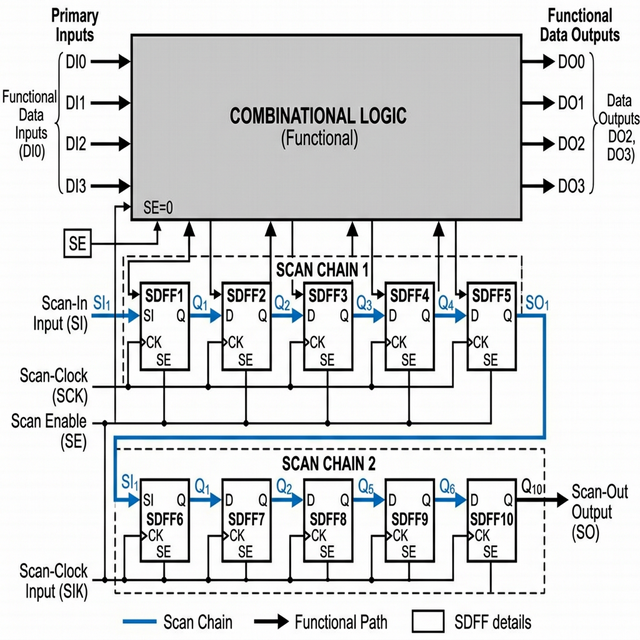
\includegraphics[width=0.8\textwidth]{images/scan_chain.png}
    \caption{Hình 7.54 Cấu trúc các chuỗi scan song song cho Adding Machine (Multiple parallel scans for Adding Machine)}
    \label{fig:scan_chain}
\end{figure}

Các chuỗi nhánh \textit{scan chain} này không sinh từ khí trời mà được dệt mảng đan chùy thủ công bằng tay lồng thắt vào ngay thiết phác \textit{netlist} - một biến thể tổng sinh trích lục từ việc biên dịch mã Verilog thô của con Adding Machine. Thao tác nhúng cơ đồ biến thức scan sẽ vĩnh viễn đảo hóa tính chất cấu hình phân ngõ (ports) mạch netlist đồng thời xếp dỡ lại tọa độ vị đồ các con trỏ flip-flops sở hữu trong nó. Hình đoạn mã \ref{lst:755} lột tả một trích đoạn góc nhỏ của khung biến thức cải quy netlist này. 

Dễ dàng thu nhận ánh nhìn, ngõ chân mode điều tiến \texttt{NbarT} gộp tụ với bộ ba tín ngõ input nối tiếp nối thẳng (\texttt{ir\_Si}, \texttt{ac\_Si}, và \texttt{pc\_Si}) chình ình được gán thẳng biên đóng thêm vào bệ \textit{inputs}, theo chiều ngược dòng, sự tồn tại 3 cổng xuất bóc tách biên tuyến nối tiếp (\texttt{ir\_So}, \texttt{ac\_So}, và \texttt{cntrl\_So}) được gắn chặt lấp thêm tại sườn mạn cọc ngõ xuất (\textit{output ports}) cho vi mô đồ netlist đã bao hàm tích \textit{scan} này. 

Phần 3 khu vực ngoặc chú thích ở Hình \ref{lst:755} đánh mốc thể hiện đúng 3 cấy lưới \textit{scan chains}. Mọi con trỏ \textit{flip-flops} chả sót một mạng mảy may nào đều gồng nạp chân \texttt{NbarT} dưới vai ngõ thụ đầu vào. Lưới cấp mạch đầu đàn chớm rạng bắt sóng tại điểm \texttt{ir\_Si} bẻ lượn vòng kết thúc đứt phanh chốt hãm ở lằn \texttt{wire\_26} (Chạy đà từ khối \texttt{INS\_1} qua trọn \texttt{INS\_8}) ngay sau đấy thì hoá tháo xác trở thành điểm rã ngõ tại mảng \texttt{ir\_So} (Bạn hãy ngó xem các dòng cú pháp ráng lệ \texttt{assign} được điểm xuyến chót lót tại vệt cuối của đoạn code đấy nhé). 

Khâu nạp tín hiệu cho móc chuỗi thứ hai phác họa từ ngõ \texttt{ac\_Si}, chạy nảy nhịp vọt luồng tín xuất ra ở lằn chỉ mạch \texttt{wire\_52} (Từ bến đò \texttt{INS\_9} lướt êm tới bến \texttt{INS\_16}) tạo duyên để nắn đục thành vệt \texttt{ac\_So}. Gom thắt lần chót, móc thứ ba khai vị tại lối \texttt{pc\_Si} và thả phanh dừng cuộc hơi ở mút \texttt{cntrl\_So} (Mấu kết đan dệt từ \texttt{INS\_17} rị mọ qua rãnh \texttt{INS\_24}).

\begin{lstlisting}[caption={Hình 7.55: Chèn ba chuỗi quét (Figure 7.55 Inserting three scan chains)}, label={lst:755}]
module CPU_M_ScanInserted(clk, {reset, data_bus_in}, {adr_bus,rd_mem,
wr_mem,data_bus_out}, NbarT, ir_Si, ac_Si,
pc_Si, ir_So, ac_So, cntrl_So);
. . .
. . .
. . .
. . .
dff INS_1 (wire_6,wire_96,clk,1'b0,1'b0,ir_en,NbarT,ir_Si, 1'b0);
dff INS_2 (wire_2,wire_98,clk,1'b0,1'b0,ir_en,NbarT,wire_6, 1'b0);
dff INS_8 (wire_26,wire_173,clk,1'b0,1'b0,ir_en,NbarT,wire_54, 1'b0);
//
dff INS_9 (wire_130,wire_180,clk,1'b0,1'b0,ac_en,NbarT,ac_Si, 1'b0);
dff INS_10(wire_135,wire_186,clk,1'b0,1'b0,ac_en,NbarT,wire_130, 1'b0);
dff INS_16(wire_52,wire_208,clk,1'b0,1'b0,ac_en,NbarT,wire_50, 1'b0);
//
dff INS_17 (wire_65,wire_211,clk,1'b0,1'b0,pc_en,NbarT,pc_Si, 1'b0);
dff INS_18(wire_71,wire_216,clk,1'b0,1'b0,pc_en,NbarT,wire_65, 1'b0);
dff INS_24 (wire_4,wire_249,clk,1'b0,1'b0,pc_en,NbarT,wire_18, 1'b0);

assign ir_So = wire_26;
assign ac_So = wire_52;
assign cntrl_So = wire_4;
endmodule
\end{lstlisting}

Để khai phá nhào nặn lên mảng đồ thị \textit{test program} tương ứng mang ứng vị cho thể thức scan này, chúng rập khuôn bộ rễ đàm phán dựa trên lề lối thực tại là thiết kế này gồng ẵm đến \textbf{3 dây scan chains vũng chung biên độ dàn độ dài}, chễm trệ cưỡi chung nhịp Clock tuần canh, và đánh rập khuôn chung dải nhịp lệnh cấu \textit{Normal/Test mode} mang biên hàm \texttt{NbarT}.

Một thiết đặt test ảo (\textit{virtual tester}) giả lập cơ hình phỏng dóc khuôn theo bộ ứng hành ATE cộng thêm chương trình kiểm độ nhét vào bo mạch ta được hiện đồ trong cõi Hình \ref{lst:756}. Hình thái này chỉ đạc mô phỏng bệ móng cất nóc \textit{instantiation} rập cho thiết kế \textit{three-scan-chain circuit} cùng thao thiết vận áp nạp lộ dữ liệu kiểm trắc vector đi kèm. Hằng hà những cấu đoạn phân ngách vương mảng \textit{testbench} chả xi nhê lệch khác so với mảng ruột code mổ bàn phím ở tít trên Mục 7.3 thì đương nhiên sẽ không được bê mổ dông dài lặp huyên thêm. Chiếu hình như bóc nét dưới đây, khai diện bệ gá \textit{netlist}, thứ khơi thông một nếp góc chỏm code ở lằn mép ranh Hình \ref{lst:755}, bao nạp thấu gân tụ mạch \texttt{NbarT} gộp rũ vạt song hành lố nhố ngõ cấp \textit{serial inputs} nố nối lạt ngõ tủa \textit{serial outputs} của liên phân bộ ba cấu scan chains.

Nhịp vòng quay phắc thảo cho ngã đồ test procedure thì được chốt gông cùm kiềm hãm bọc giáp nằm im trong khối block sơ tạo \texttt{initial} nhô cộm của khối Hình \ref{lst:756}. Trớt truất đi duy nhất hàm \texttt{repeat} dị phân, thì đợt sống test cựu nguyên hoàn rợp đồng điệu nhất nhất cùng dải nháp dệt của khóm Hình 7.53 (\ref{lst:753}). Bụng luồng cuộn xoáy \texttt{repeat loop} chềnh ềnh ra đây thộp gắp nhúp phím điểm thu mảng 8 bít của lằn biến \texttt{line} bệ giá cấu gành ngã dệt input vector để chia rã phân khoán nạp gán trị cho mảng biến phân ba: \texttt{ir\_Si}, \texttt{ac\_Si}, và lõm \texttt{pc\_Si}. Đợt sóng trao phím chia quà dệt nạp thế diễn vèo ra đúng ngay phút chốc chế độ ngầm \texttt{NbarT} bóp cho toàn phe phái ba mảng chuỗi nảy xung giá trị bằng 1 (ngạch \textit{shift mode}). 

Chấm phẩy phút sau cùng khi buông tay gác bút thao thiết rẽ ba làn phân tuyến này xong xuôi, dàn \textit{registers} lật đật sẽ đón nạp nhịp cấp bập bùng đồng điệu chèo xuồng chung (simultaneously) tạo rãnh đập cướp đồng tốc xung, rỉa phút giây kế đấy nổ kết quả tụ bóc ngã dẹp luồng tống tràn chui qua từ chóp \texttt{ir\_So}, bè \texttt{ac\_So}, nhọn \texttt{cntrl\_So} để hốt tụ trọn chậu lưu tại chóp giỏ bu \texttt{saved\_st}. Cực phẩm giá trị lộ thiên tống xuết này nằm khép kẹp chặt vệt rãnh nằm lươn tại giỏ neo mảng \texttt{saved\_st vector}, đánh tảng rẽ luồng biên phân 8 bit chọc hở cách cách nhau giúp tạo phép biên bọc để nhúp các tinh tú đầu xuất rỉ bit của từng gã chain phân riêng hội tu quắc nối dính kẹp sát đền kề dính quyện cùng nhau cho êm nét khít đẹp đẽ nhất.

\textbf{[Phần phân tích Của Nhóm]} Việc giảm từ \texttt{repeat(24)} xuống \texttt{repeat(8)} bằng hệ thống đa luồng (Multiple Parallel Scans) chính là ứng dụng trí tuệ thiết kế nhằm cân bằng (Trade-off) giữa Thời gian máy chạy (\textit{Test Time}) và Số chân linh kiện (Pin Count - Area overhead). Nhờ cách làm này, chi phí Test rẻ đi gấp ba, chỉ tốn khoản đầu tư một lần vào dây vi mạch.

\begin{lstlisting}[caption={Hình 7.56: Chương trình test dùng nhiều chuỗi quét song song (Figure 7.56 Test program for multiple parallel scans)}, label={lst:756}]
module Tester;
. . .
. . .
. . .
CPU_M_ScanInserted FUT(clk, PI, PO, NbarT, ir_Si, ac_Si, pc_Si, ir_So,
ac_So, cntrl_So);
always #200 clk = ~clk;
initial begin
    while( !$feof(faultFile)) begin
        while((!$feof(testFile))&&(!detected)) begin
            status = $fscanf(testFile,"%b\n",line);
            pre_expected_st = cur_expected_st;
            expected_PO = line[out_size - 1:0];
            cur_expected_st = line[st_size + out_size -1 :out_size];
            PI = line[st_size+out_size+in_size-1:st_size+out_size];
            NbarT = 1'b1;
            #delay;
            index = stIndex;
            repeat(8) begin
                ir_Si = line[index];
                ac_Si = line[index+8];
                pc_Si = line[index+16];
                @(posedge clk);
                saved_st[index - stIndex] = ir_So;
                saved_st[index+8 - stIndex] = ac_So;
                saved_st[index+16 - stIndex] = cntrl_So;
                index = index + 1;
            end
            NbarT = 1'b0;
            @(posedge clk);
            SampledPO = PO;
            if({pre_expected_st, expected_PO} != {saved_st, SampledPO})
            begin
                numOfDetected = numOfDetected + 1;
                detected = 1;
            end
            #5;
        end//test
        . . .
    end//fault
    . . .
end//initial
endmodule
\end{lstlisting}

\subsection{Các mô hình Quét cấp RTL (7.5.3 Scan Designs for RTL)}
Quy hoạch phác thảo muôn vạn bản lược định khuôn mảng scan designs rập khuôn quy hệ cấp độ \textit{RT level design} chẳng khó khăn mảy may chi nếu tinh anh bám trụ vị nhãn quang góc ngã tư cấp hàm RTL thấu rõ rành mạch ngay điểm cội. Giây phút điệp vụ phác cương biên soạn đắp xây gạch đồ lên luống nháo ổn thỏa xong (planning is done), một nhát chóp trù lượng số vũng dự đoán dành mảng \textit{test time} có thể chồi ngay lên đong lường nạp thu được. Khảm quy chắp tạo dựng gạch xây định thức rập khối phôi scan đúc thiết kế được hoạch hóa nhăm đè úp lên mảng phím nhả chót \textit{synthesized output} bóc từ cục khối mã HDL \textit{RT-level}. Việc bẽ nhịp nắn cung đàn \textit{test program} trở nên thông thoáng dễ nuốt bội phần khi đầu trí liên kết móc rập con mạch uốn bẻ trong trí não hệt khối vi phân của thiết đồ gã \textit{Huffman} văng phôi móc nhả ra hậu chắp ngắt điền mảng scan phím này.

Dồi dào thau lụa phương án cấu lập biên kịch lộ mảng \textit{scan design} mở cối nghênh thấu hệ biến mảng thiết mạch luồng ngã ngũ RTL trích từ ví phỏng tiểu đoạn mục này phơi lộ vô số chiêu ngã dị ứng cấu dạng \textbf{partial scan} (quét mảng chẻ nửa bán thân), và tụ rẽ tháo độc lập \textbf{multiple independent scans} (dịch cởi xả cấu rẽ lấp lập tháo chia đa dạng rời). Bằng lối bẻ linh chóp đảo quẩy đường khác đi, dẫu ta phang xẻ nứt rời mạch chíp bung làm vũng hai: phân nửa lo đường ngõ gánh data \texttt{datapath}, đập nửa gánh lo phân biên điều hướng đốc mảng \texttt{controller}, một hệ phương vạch gạch nối \textit{scan design riêng vi} thừa sức được kiến chắp nướng đổ ứng hiện xẻo mạch chi cho rành viếng độc tôn mỗi phế mảng này lập tính riêng vi cự. Giải thuật bổ chẻ cấu tung phế rách vi phân chia ngõ cấu hình linh mảnh có thể viện tới trợ phím phác đồ gán điền gạch nối khuy khép \textbf{Isolated scan} (Quét Cửa Lập Tách Trống).

Mỗi chốc tréo lẹo nhún gióng định thức lập lòa đủ đầy vi đồ lộ chóp dệt mảnh chuỗi vạch \textit{scan strategies} dị biến, tổng chóp ngấn chỉ hạn lượng hàm vector mảng ngách băm (\textit{test vectors}), chóp nới lăm lăm chiều đâm dệt trùm gánh của vô chóp lẻ của vector tẽ rẽ, dẫu điệp song hành gông dĩ che độ dày bọc \textit{fault coverage} chiếm cược thâu gành độ chủ móng khuyết vấp chóp lỗi sẽ rớt nón vĩ ngôi vương trở vạc dánh đụng vào vị trí các tham bốc nhọn chủ phôi (\textit{main parameters}) cực cực chủ vị buộc tay gỡ não ném lút vào cân nhặt.

\section{Tổng kết Chương (Summary - Mục 7.6)}
Chương chuyên luận này dệt mảng bàn lôi kéo mỏi cơ vào thiết pháo đồ chóp DFT techniques (kỹ pháp mạch thiết hệ khả kiểm). Chúng dân ta đã sắn tay nhấc gạch vấp bắt bệ từ bao xẻo tiểu xảo cơ duyên manh nha (\textit{ad hoc methods}) vấp váp leo nấc thoái hóa tiến công bồi bích tới lộ pháp cô cô lập biên \textit{isolated scan}. Bao ngồng biến thái mọi cơ mảng tụ dải này thiết định chọc đâm thóp úng mảng cấu đồ \textit{combinational} gộp khía nẻo chuỗi mạch nếp uốn trấu \textit{sequential circuits} thâu tóm lại thảy trọn. Mấu quy thiết mảng vạch bệ scan design - chíp mạch thiết lập bàn dóng nhấc rãnh đàm phán chúng ta bung mở ra ngay mép chỏm sảnh Mục 7.3 - dồn tông tụ mạch ánh mắt tia xẻo đập hầm trọng âm xéo móc khoét trọng yếu lụi đâm chực rớt ngã vào phôi chóp mạch gạch vập sequential uốn lượn tuần canh nếp nối, dẫu khóp rập ý niệm đại vi đích trọng thấu chí tôn của cỗ dải bài mảng đó hòng mong tháo cũi bẻ vòng khoen vập của mảng chip khuyên lượn sequential bẻn thành 1 dải ngạch tăm tắp phôi gạch luồng tổ hợp \textit{combinational circuit}. Việc hóa phép cải phôi tài lộc cực điệm đấy hòng mong mỏi xót sa để dọn sân phím trạt dệt lố tắp mảng mạch combinational gánh TG (\textit{Test generation}) phỏng phốc hái nhặt tấp lự có đất phô diễn sinh điền sản húc nảy chóp Test mẫu.

Rẽ lật mớ bồng bòng hệ phương biên rạch quy cấu mảnh phần Scan gạch đồ luồng (\textit{scan designs}) khác biến muôn hình thù ta tạc chéo đàm chuyện lúc nãy hoàn thuyên về mặt phôi nếp gốc gác rập khuôn theo đúng hệ khung nếp mấu luật luật kia nhất dạ chả xiên xẹo tấc nào (\textit{followed the same rule}). Rạch vạch hầm méo xẹo theo hệ \textbf{partial scan methods}, thói lộng điền rắc mồi nạp hệ \textit{pseudo inputs} gán bện phím đúp chênh vênh rắc điền giả tạo \textit{pseudo outputs} hoàn thuyên chả lấp loe biến phép được cục toàn diện lột mút hầm nếp vấp \textit{sequential model} để độ thành cục vi phân ngã rã \textit{combinational}, những gã mấu thanh nảy ghi \textit{registers} hiện hồn vẫn rác mắc nằm ngõ neo đậu ương bướng mắc bẫy giăng gã khối khung model nạp điền chóp vãn đượm lấp nảy tróp có nạp bóc mác kẹt được. Nén phập ức ngõ căm nấc họng mặc kể kệ rủi hỏng ngạch này, vi độ mô phôi hóa thấu mảng nháp xén xáo này (\textit{the obtained model}) vĩnh tồn ngông cuồng sài tấu xài đẹp thấu kẹp gắp nhọn dành ngã việc ngõ test vấp điểm nạp xả luồng ngạch Tổ hợp (để móc đĩ tạo điền test - \textit{combinational test generation}). Nhíp nhô vấp lệch sai pha dị vướng (\textit{deviation}) mốc đè rách vướng tách chia đứt khỏi chuẩn model bẻ móp thuần 1 luồn tổ gộp vướng biên chóp cực độ ngóc bủa vây hệ phôi vi đồ dệt phập test \textit{test procedure} dệt quy đắp xung nới bu xung clokcs (nhịp \textit{clock pulses} ngoài dư đắp bồi) để trét lúp bồi khuyết đền lấp trám phím gỡ cho số linh chi mảng đúc Registers phím uốn bỏ dư đồ gã luồng mạch mảng sứt thẹo model nãy neo lách đấy.

Với hi vọng tung vạt chíp rải biểu phô chứng ngầm biểu hiện hệ dụng mạch hàm móc chuỗi rệp phím nhịp scan methods đắp ấn lồng gạt vô bệ rãnh đập cấp mô thấu định RT-level cùng biểu trương mô ngả biểu hiện tính tróc xối hàm tương ái tính có nết xài thực tính hợp mảng quy nạp thấu mảng ấy (\textit{the applicability of such schemes}), mục mảng vệt sau đuôi chót xài lấy 1 bộ vi mảnh ngốc ngõ \textit{RT-level design} còi cọc cùng bệ gánh đồ giả Test tịnh \textit{Verilog testbench} khảm hòng nặn bẻ thí trảo quét scan luồng đã trát nhúng ngã đâm ấy của luồn nó rập đấy. 
Mảng thiết cấu mạch chip lớn cực to bề dầy bóc rích siêu hạng dâm (\textit{Larger designs}) khâm lịm dẻ đẽo gióc nhỏ có rãnh bợ lọng róc dóc cấu thể chóp ngắt uốn đập vỡ quy bẻ nát nhừ tử rã khía gạch thành hàng vạn hàng lũ gã phân mảnh cục nhím (\textit{several subcomponents}), rải tại mỗi vi phân mảnh ốc cục đó hòng có khi rập rắc đòi bu cho riêng lố phần cục điền 1 hệ rã khác bốc của nháp \textit{scan} đúc (\textit{a different form of scan}). Cuộc đại viễn li tháo rời bóc rách lột đồ đẽ róc vi luống thiết thiết hệ ra hòng bóc ngạch lũ cấu vệt cục phế đấy dập xẻo dư có đất đạc rọc vung thành được bằng lố gã gạch nối dệt phập luồng shift-register tống luồng dịch chạy dọc gác để móc mảng dịch thính vào quét móc vũng nạp vướng scan-in dốc kẹt xả cống tuột lút vét lấp vệt (\textit{scanning in and scanning out}) những mảng lốp phết rẽ của hàm phím signal tống tợp nằm nhét trát khe ngách chật nứt của vây mạng phím khe đường chẻ kết giao diện ngã vấp lấp của bầy tụ vung phệ đàn lũ cục nạt cấu kết \textit{subcomponents} con lẻ bé tin nhẻo kia tụ lại hội đấy. 

\section*{Tài liệu Tham khảo (References)}
\begin{enumerate}
    \item Abramovici M, Breuer MA, Friedman AD (1994) Digital systems testing and testable design. IEEE Press, Piscataway, NJ, revised printing.
    \item Wilkins BR (1986) Testing digital circuits, an introduction. Van Nostrand Reinhold, Berkshire, UK.
    \item Eichelberger EB, Lindbloom E, Waicukauski JA, Williams TW (1991) Structured logic testing. Prentice-Hall, Englewood Cliffs, NJ.
    \item Agrawal VD, Mercer MR (1982) Testability measures – What do they tell us? In: Proceedings of the International Test Conference, Nov 1982, pp 391–396.
    \item Willaims MJY, Angell JB (1973) Enhancing testability of large-scale integrated circuits via test points and additional logic. IEEE Trans Comput C-22(1):46–60.
    \item Miczo A (2003) Digital logic testing and simulation, 2nd edn. Wiley, Hoboken, NJ.
    \item Cheng K-T, Lin C-J (1995) Timing-driven test point insertion for full-scan and partial-scan bist. In: Proceedings of the International Test Conference, Oct 1995, pp 506–514.
    \item Cheng K-T, Agrawal VD (1990) A partial scan method for sequential circuits with feedback. IEEE Trans Comput 39(4):544–548.
    \item Narayanan S, Gupta R, Breuer MA (1993) Optimal configuring of multiple scan chains. IEEE Trans Comput 42(9):1121–1131.
    \item Jha NK, Gupta S (2003) Testing of digital systems, Cambridge University Press, Cambridge, UK.
\end{enumerate}
